\documentclass[DaoFP]{subfiles}
\begin{document}
\setcounter{chapter}{8}

\chapter{自然变换}

我们已经看到,当两个对象 $a$ 和 $b$ 是同构的时,它们会在箭头集合之间产生双射,我们现在可以将其表示为 hom-集之间的同构。对于所有 $x$,我们有:
\begin{align*}
\mathcal{C}(a, x) &\cong \mathcal{C}(b, x) \\
\mathcal{C}(x, a) &\cong \mathcal{C}(x, b)
\end{align*}
然而,反过来并不成立。除非满足额外的自然性条件,否则 hom-集之间的同构不会导致对象之间的同构。我们现在将在逐步更一般的设置中重新表述这些自然性条件。

\section{Hom-函子之间的自然变换}

建立两个对象之间同构的一种方法是直接提供两个箭头——一个作为另一个的逆。但通常更简单的方法是间接地通过定义箭头之间的双射来实现,无论是作用于这两个对象的箭头,还是从这两个对象发出的箭头。

例如,正如我们之前所见,对于每个 $x$,我们可能有一个可逆的箭头映射 $\alpha_x$。
\[
 \begin{tikzcd}
 \node(x) at (0, 2) {x};
 \node(a) at (-2, 0) {a};
 \node(b) at (2, 0) {b};
 \node(c1) at (-1, 1.5) {};
 \node(c2) at (-1.5, 1) {};
 \node(c3) at (-1, 2) {};
 \node(c4) at (-2, 1) {};
 \node(d1) at (1, 1.5) {};
 \node(d2) at (1.5, 1) {};
 \node(d3) at (1, 2) {};
 \node(d4) at (2, 1) {};
\node (aa) at (-1, 0.75) {};
 \node (bb) at (1, 0.75) {};
 \draw[->] (x) .. controls (c1)  and (c2) .. (a); % bend
 \draw[->, green] (x) .. controls (c3)  and (c4) .. (a); % bend
 \draw[->, blue] (x) -- (a); 
  \draw[->] (x) .. controls (d1)  and (d2) .. (b); % bend
 \draw[->, green] (x) .. controls (d3)  and (d4) .. (b); % bend
 \draw[->, blue] (x) -- (b); 
 \draw[->, red, dashed] (aa) -- node[above]{\alpha_x} (bb);
 \end{tikzcd}
\]
换句话说,对于每个 $x$,存在一个 hom-集的映射:
\[ \alpha_x \colon \mathcal{C}(x, a) \to \mathcal{C}(x, b) \]

当我们变化 $x$ 时,这两个 hom-集成为两个(逆变)函子,$\cat C(-, a)$ 和 $\cat C(-, b)$,而 $\alpha$ 可以看作它们之间的映射。这样的函子映射,称为变换,实际上是一系列单独的映射 $\alpha_x$,每个对象 $x$ 在范畴 $\mathcal{C}$ 中都有一个。

函子 $\mathcal{C}(-, a)$ 描述了世界看待 $a$ 的方式,而函子 $\mathcal{C}(-, b)$ 描述了世界看待 $b$ 的方式。

变换 $\alpha$ 在这两种视图之间来回切换。$\alpha$ 的每个组成部分,即双射 $\alpha_x$,表明从 $x$ 看 $a$ 的视图与从 $x$ 看 $b$ 的视图是同构的。

我们之前讨论的自然性条件是:

\[ \alpha_y \circ (- \circ g) = (- \circ g) \circ \alpha_x \]
它关联了在不同对象处取的 $\alpha$ 的组成部分。换句话说,它关联了两个不同观察者 $x$ 和 $y$ 的视图,这两个观察者通过一个箭头 $g \colon y \to x$ 连接。

这个等式的两边都作用于 hom-集 $\mathcal{C}(x, a)$。结果在 hom-集 $\mathcal{C}(y, b)$ 中。我们可以将两边重写为:
\begin{align*}
 \cat C(x, a) \xrightarrow{(- \circ g)} \cat C(y, a) \xrightarrow{\alpha_y} \cat C(y, b) \\
\cat C(x, a) \xrightarrow{\alpha_x}  \cat C(x, b)  \xrightarrow{(- \circ g)}\cat C(y, b)
\end{align*}

与 $g \colon y \to x$ 的预组合也是 hom-集的映射。事实上,它是通过逆变 hom-函子提升的 $g$。我们可以分别将其写为 $\mathcal{C}(g, a)$ 和 $\mathcal{C}(g, b)$。
\begin{align*}
 \cat C(x, a) \xrightarrow{\cat C(g, a)} \cat C(y, a) \xrightarrow{\alpha_y} \cat C(y, b) \\
\cat C(x, a) \xrightarrow{\alpha_x}  \cat C(x, b)  \xrightarrow{\cat C(g, b)}\cat C(y, b)
\end{align*}

因此,自然性条件可以重写为:
\[ \alpha_y \circ \mathcal{C}(g, a) = \mathcal{C}(g, b) \circ \alpha_x \]
它可以通过以下交换图来说明:
\[
 \begin{tikzcd}
 \mathcal{C}(x, a)
 \arrow[d, "\alpha_x"]
 \arrow[r, "{\mathcal{C}(g, a)}"]
 &
 \mathcal{C}(y, a)
  \arrow[d, "\alpha_y"]
 \\
 \mathcal{C}(x, b)
 \arrow[r, "{\mathcal{C}(g, b)}"]
& \mathcal{C}(y, b)
 \end{tikzcd}
\]

我们现在可以重新表述我们之前的结果:满足自然性条件的函子 $\mathcal{C}(-, a)$ 和 $\mathcal{C}(-, b)$ 之间的可逆变换 $\alpha$ 等价于 $a$ 和 $b$ 之间的同构。

我们可以对出射箭头进行完全相同的推理。这次我们从一个变换 $\beta$ 开始,其组成部分为:
\[ \beta_x \colon \mathcal{C}(a, x) \to \mathcal{C}(b, x) \]
两个(协变)函子 $\mathcal{C}(a, -)$ 和 $\mathcal{C}(b, -)$ 分别描述了从 $a$ 和 $b$ 的角度看待世界的方式。可逆变换 $\beta$ 告诉我们这两种视图是等价的,而自然性条件
\[ (g \circ -) \circ \beta_x = \beta_y \circ (g \circ -) \]
告诉我们当我们切换焦点时它们表现良好。

以下是说明自然性条件的交换图:
\[
 \begin{tikzcd}
 \mathcal{C}(a, x)
 \arrow[d, "\beta_x"]
 \arrow[r, "{\mathcal{C}(a, g)}"]
 &
 \mathcal{C}(a, y)
  \arrow[d, "\beta_y"]
 \\
 \mathcal{C}(b, x)
 \arrow[r, "{\mathcal{C}(b, g)}"]
& \mathcal{C}(b, y)
 \end{tikzcd}
\]

同样,这样的可逆自然变换 $\beta$ 建立了 $a$ 和 $b$ 之间的同构。

\section{函子间的自然变换}

上一节中的两个hom-函子为
\begin{align*}
 F x &=   \mathcal{C}(a, x) \\
G x &=   \mathcal{C}(b, x)
\end{align*}
它们都将范畴$\mathcal{C}$映射到$\mathbf{Set}$,因为hom-集存在于$\mathbf{Set}$中。我们可以说它们在$\mathbf{Set}$内创建了$\mathcal{C}$的两个不同\emph{模型}。

自然变换是这两个模型之间的结构保持映射。
\[
 \begin{tikzcd}
 && \cat C(a, x)
 \arrow[dd, "\beta_x"]
 \\
 x
 \arrow[rru, dashed, "{\cat C(a, -)}"]
 \arrow[rrd, dashed, "{\cat C(b, -)}"']
 \\
 && \cat C(b, x)
 \end{tikzcd}
\]

这一思想自然地扩展到任意一对范畴之间的函子。任意两个函子
\begin{align*}
F &\colon \mathcal{C} \to \mathcal{D} \\
G &\colon \mathcal{C} \to \mathcal{D}
\end{align*}
都可以看作$\mathcal{C}$在$\mathcal{D}$内的两个不同模型。

为了将一个模型转换为另一个模型,我们使用$\mathcal{D}$中的箭头连接对应的点。对于$\mathcal{C}$中的每个对象$x$,我们选择一个从$F x$到$G x$的箭头:
\[ \alpha_x \colon F x \to G x \]
因此,自然变换将对象映射为箭头。
\[
 \begin{tikzcd}
 && F x
 \arrow[dd, "\alpha_x"]
 \\
 x
 \arrow[rru, dashed, "F"]
 \arrow[rrd, dashed, "G"']
 \\
 && G x
 \end{tikzcd}
\]

然而,模型的结构不仅与对象有关,还与箭头有关,因此让我们看看箭头会发生什么。对于$\mathcal{C}$中的每个箭头$f \colon x \to y$,我们在$\mathcal{D}$中有两个对应的箭头:
\begin{align*}
 F f &\colon F x \to F y \\
G f &\colon G x \to G y 
\end{align*}
这是$f$的两个提升。我们可以用它们在两个模型的边界内移动。然后还有$\alpha$的分量,它们让我们在模型之间切换。

自然性意味着,无论你是先在第一个模型内移动然后跳到第二个模型,还是先跳到第二个模型然后在其中移动,都不应该有区别。这由交换的\emph{自然性方块}说明:

\[
 \begin{tikzcd}
 F x
 \arrow[d, "\alpha_x"]
 \arrow[r, "F f"]
 &
F y
  \arrow[d, "\alpha_y"]
 \\
G x
 \arrow[r, "G f"]
& G y
 \end{tikzcd}
\]

满足自然性条件的这样一族箭头$\alpha_x$被称为\emph{自然变换}。

这是一个展示一对范畴、它们之间的两个函子以及函子之间的自然变换$\alpha$的图表:
\[
\begin{tikzcd}[column sep=huge]
\mathcal{C}
  \arrow[bend left=50]{r}[name=U, label=above:$F$]{}
  \arrow[bend right=50]{r}[name=D, label=below:$G$]{} 
 &
\mathcal{D}
  \arrow[shorten <=10pt,shorten >=10pt,Rightarrow,to path={(U) -- node[label=left:$\alpha$] {} (D)}]{}
\end{tikzcd}
\]

由于对于$\mathcal{C}$中的每个箭头都有一个对应的自然性方块,我们可以说自然变换将对象映射为箭头,将箭头映射为交换方块。

如果自然变换的每个分量$\alpha_x$都是同构,则$\alpha$被称为\emph{自然同构}。

我们现在可以重新表述关于同构的主要结果:两个对象是同构的,当且仅当它们的hom-函子之间存在自然同构(无论是协变还是反变函子——任何一个都可以)。

自然变换提供了一种非常方便的高层次方式来表达各种情况下的交换条件。我们将利用这种能力重新表述代数数据类型的定义。


\section{编程中的自然变换}

自然变换是由对象参数化的一族箭头。在编程中,这对应于由类型参数化的一族函数,即\emph{多态函数}。

自然变换的参数类型由一个函子描述,返回类型由另一个函子描述。

在Haskell中,我们可以定义一个数据类型,它接受两个表示两个函子的类型构造器,并生成自然变换的类型:

\begin{haskell}
data Natural :: (Type -> Type) -> (Type -> Type) -> Type where
  Natural :: (forall a. f a -> g a) -> Natural f g
\end{haskell}
\hask{forall}量词告诉编译器该函数是多态的——即,它为每个类型\hask{a}定义。只要\hask{f}和\hask{g}是函子,这个公式就定义了一个自然变换。

由\hask{forall}定义的类型非常特殊。它们在\index{参数多态}\emph{参数多态}的意义上是多态的。这意味着一个公式适用于所有类型。我们已经看到了恒等函数的例子,它可以写成:
\begin{haskell}
id :: forall a. a -> a
id x = x
\end{haskell}
这个函数的主体非常简单,只是变量\hask{x}。无论\hask{x}是什么类型,公式都保持不变。

这与\index{特设多态}\emph{特设多态}形成对比。特设多态函数可能为不同类型使用不同的实现。这种函数的一个例子是\hask{fmap},它是\hask{Functor}类型类的成员函数。对于列表有一个\hask{fmap}的实现,对于\hask{Maybe}有另一个实现,依此类推,逐个案例。

Haskell中(参数)自然变换的标准定义使用\emph{类型同义词}:
\begin{haskell}
type Natural f g = forall a. f a -> g a
\end{haskell}
\index{\hask{type}同义词}\hask{type}声明为右侧引入了一个别名,一个简写。

事实证明,将自然变换的类型限制为参数多态具有深远的影响。这样的函数自动满足自然性条件。这是\index{参数性}参数性产生所谓\index{免费定理}\emph{免费定理}的一个例子。

我们无法在Haskell中表达箭头的等式,但我们可以使用自然性来转换程序。特别是,如果\hask{alpha}是一个自然变换,我们可以将:
\begin{haskell}
fmap h . alpha
\end{haskell}
替换为:
\begin{haskell}
alpha . fmap h
\end{haskell}
在这里,编译器会自动确定使用哪个版本的\hask{fmap}和\hask{alpha}的哪些组件。

我们还可以使用更高级的语言选项来明确选择。我们可以使用一对函数来表达自然性:
\begin{haskell}
oneWay :: 
  forall f g a b. (Functor f, Functor g) => 
  Natural f g -> (a -> b) -> f a -> g b
oneWay alpha h = fmap @g h . alpha @a
\end{haskell}
\begin{haskell}
otherWay :: 
  forall f g a b. (Functor f, Functor g) => 
  Natural f g -> (a -> b) -> f a -> g b
otherWay alpha h = alpha @b . fmap @f h
\end{haskell}
注释\hask{@a}和\hask{@b}指定了参数多态函数\hask{alpha}的组件,注释\hask{@f}和\hask{@g}指定了特设多态\hask{fmap}实例化的函子。

这是一个有用的函数的例子,它是列表函子和\hask{Maybe}函子之间的自然变换:
\begin{haskell}
safeHead :: Natural [] Maybe
safeHead [] = Nothing
safeHead (a : as) = Just a
\end{haskell}
(标准库中的\hask{head}函数是“不安全的”,因为它在给定空列表时会出错。)

另一个例子是函数\hask{reverse},它反转一个列表。它是列表函子到列表函子的自然变换:
\begin{haskell}
reverse :: Natural [] []
reverse [] = []
reverse (a : as) = reverse as ++ [a]
\end{haskell}
顺便说一下,这是一个非常低效的实现。实际的库函数使用了优化的算法。

理解自然变换的一个有用直觉是建立在函子像数据容器的想法上的。你可以对容器做两件完全正交的事情:你可以转换它包含的数据,而不改变容器的形状。这就是\hask{fmap}所做的。或者你可以将数据转移到另一个容器中,而不修改它。这就是自然变换所做的:它是一种在容器之间移动“东西”的过程,而不知道“东西”是什么类型。

换句话说,自然变换将一个容器的内容重新打包到另一个容器中。它以对内容类型不可知的方式进行,这意味着它不能检查、创建或修改内容。它所能做的就是将其移动到新位置,或丢弃它。

自然性条件强制了这两个操作的正交性。无论你是先修改数据然后将其移动到另一个容器中,还是先移动它然后修改,都没有关系。

这是将复杂问题成功分解为一系列简单问题的另一个例子。不过,请记住,并非所有涉及数据容器的操作都可以以这种方式分解。例如,过滤需要检查数据,以及改变容器的大小甚至形状。

另一方面,几乎每个参数多态函数都是自然变换。在某些情况下,你可能需要考虑恒等函子或常函子作为源或目标。例如,多态恒等函数可以被视为两个恒等函子之间的自然变换。

\subsection{自然变换的垂直复合}

自然变换只能在\emph{平行}函子之间定义,即共享相同源类别和相同目标类别的函子。这样的平行函子形成一个\emph{函子类别}。两个类别$\mathcal{C}$和$\mathcal{D}$之间的函子类别的标准表示法是$[\mathcal{C}, \mathcal{D}]$。你只需将两个类别的名称放在方括号之间。

$[\mathcal{C}, \mathcal{D}]$中的对象是函子,箭头是自然变换。

为了证明这确实是一个类别,我们必须定义自然变换的复合。如果我们记住自然变换的组件是目标类别中的常规箭头,这就很容易了。这些箭头可以复合。

确实,假设我们有一个在两个函子$F$和$G$之间的自然变换$\alpha$。我们想将其与另一个从$G$到$H$的自然变换$\beta$复合。

\[
\begin{tikzcd}[column sep=huge]
\mathcal{C}
  \arrow[bend left=60]{rr}[name=U, label=above:$F$]{}
  \arrow[]{rr}[name=M, label={[xshift=15pt, yshift=-5pt]:$G$}]{} 
  \arrow[bend right=60]{rr}[name=D, label=below:$H$]{} 
 &&
\mathcal{D}
  \arrow[shorten <=8pt, shorten >=8pt,Rightarrow, to path={(U) -- node[label=left:$\alpha$] {} (M)}]{}
  \arrow[shorten <=8pt, shorten >=8pt,Rightarrow, to path={(M) -- node[label=left:$\beta$] {} (D)}]{}
\end{tikzcd}
\]

让我们看看这些变换在某个对象$x$处的组件
\[ \alpha_x \colon F \, x \to G \, x \]
\[ \beta_x \colon G \, x \to H \, x \]
这些只是$\mathcal{D}$中的两个可复合的箭头。所以我们可以定义一个复合自然变换$\gamma$如下:
\[ \gamma \colon F \to H\]
\[ \gamma_x = \beta_x \circ \alpha_x \]
这被称为自然变换的\emph{垂直复合}。你会看到它用点$\gamma = \beta \cdot \alpha$或简单的并置$\gamma = \beta \alpha$表示。

$\gamma$的自然性条件可以通过将$\alpha$和$\beta$的两个自然性方块垂直粘贴在一起来展示:
\[
 \begin{tikzcd}
 F x
 \arrow[d, "\alpha_x"]
 \arrow[r, "F f"]
 \arrow[dd, bend right = 60, "\gamma_x"']
 &
F y
  \arrow[d, "\alpha_y"]
 \arrow[dd, bend left = 60, "\gamma_y"]
 \\
G x
 \arrow[r, "G f"]
 \arrow[d, "\beta_x"]
& G y
\arrow[d, "\beta_y"]
\\
H x
\arrow[r, "H f"]
& H y
 \end{tikzcd}
\]

在Haskell中,自然变换的垂直复合只是应用于多态函数的常规函数复合。使用自然变换在容器之间移动项目的直觉,垂直复合将两个这样的移动一个接一个地组合起来。

\subsection{函子范畴}

由于自然变换的复合是通过箭头的复合来定义的,因此它自动满足结合律。

对于每个函子$F$,还存在一个恒等自然变换$id_F$。它在$x$处的分量是对象$F x$上的通常恒等箭头:
\[ (id_F)_x = id_{F x} \]

总结来说,对于每一对范畴$\mathcal{C}$和$\mathcal{D}$,存在一个函子范畴$[\mathcal{C}, \mathcal{D}]$,其中自然变换作为箭头。

该范畴中的hom-set是两个函子$F$和$G$之间的自然变换的集合。按照标准的符号约定,我们将其写为:
\[ [\mathcal{C}, \mathcal{D}](F, G) \]
其中范畴的名称后跟括号中的两个对象(此处为函子)的名称。

在范畴论中,对象和箭头的表示方式不同。对象用点表示,箭头用带尖的线表示。

在$\mathbf{Cat}$(范畴的范畴)中,函子被表示为箭头。但在函子范畴$[\cat C, \cat D]$中,函子被表示为点,而自然变换被表示为箭头。

在一个范畴中的箭头,在另一个范畴中可能成为对象。


\begin{exercise}
证明自然变换复合的自然性条件:
\[ \gamma_y \circ F f = H f \circ \gamma_x \]
提示:使用$\gamma$的定义以及$\alpha$和$\beta$的两个自然性条件。
\end{exercise}

\subsection{自然变换的水平复合}

自然变换的第二种复合方式是由函子的复合诱导的。假设我们有一对可复合的函子
\begin{align*}
 F \colon \mathcal{C} \to \mathcal{D}
&&G \colon \mathcal{D} \to \mathcal{E} 
\end{align*}
同时,还有另一对可复合的函子:
\begin{align*}
 F' \colon \mathcal{C} \to \mathcal{D}
&& G' \colon \mathcal{D} \to \mathcal{E} 
\end{align*}
我们还有两个自然变换:
\begin{align*}
\alpha \colon F \to F'  
&& \beta \colon G \to G' 
\end{align*}
图示如下:
\[
\begin{tikzcd}[column sep=huge]
\mathcal{C}
  \arrow[bend left=50]{r}[name=U, label=above:$F$]{}
  \arrow[bend right=50]{r}[name=D, label=below:$F'$]{} 
 &
\mathcal{D}
  \arrow[bend left=50]{r}[name=U1, label=above:$G$]{}
  \arrow[bend right=50]{r}[name=D1, label=below:$G'$]{} 
 &
\mathcal{E}
  \arrow[shorten <=10pt,shorten >=10pt,Rightarrow,to path={(U) -- node[label=left:$\alpha$] {} (D)}]{}
  \arrow[shorten <=10pt,shorten >=10pt,Rightarrow,to path={(U1) -- node[label=left:$\beta$] {} (D1)}]{}
\end{tikzcd}
\]
\emph{水平复合} $\beta \circ \alpha$ 将 $G \circ F$ 映射到 $G' \circ F'$。
\[
\begin{tikzcd}[column sep=huge]
\mathcal{C}
  \arrow[bend left=50]{r}[name=U, label=above:$G \circ F$]{}
  \arrow[bend right=50]{r}[name=D, label=below:$G' \circ F'$]{} 
 &
\mathcal{E}
  \arrow[shorten <=10pt,shorten >=10pt,Rightarrow,to path={(U) -- node[label=left:$\beta \circ \alpha$] {} (D)}]{}
\end{tikzcd}
\]

让我们选取 $\mathcal{C}$ 中的一个对象 $x$,并尝试定义复合 $(\beta \circ \alpha)$ 在 $x$ 处的分量。它应该是 $\cat E$ 中的一个态射:
\[ (\beta \circ \alpha)_x \colon G ( F x) \to G' ( F' x) \]

我们可以使用 $\alpha$ 将 $x$ 映射到一个箭头
\[ \alpha_x \colon F x \to F' x \]
我们可以使用 $G$ 将这个箭头提升
\[ G (\alpha_x) \colon G (F x) \to G (F' x) \]
为了从那里到达 $G' (F' x)$,我们可以使用 $\beta$ 的适当分量
\[ \beta_{F' x} \colon G (F' x) \to G' (F' x) \]
总的来说,我们有
\[ (\beta \circ \alpha)_x = \beta_{F' x} \circ G (\alpha_x) \]

但还有另一个同样合理的候选:
\[ (\beta \circ \alpha)_x = G'(\alpha_x) \circ \beta_{F x}\]
幸运的是,由于 $\beta$ 的自然性,它们是相等的。

\[
 \begin{tikzcd}
  && G(F x)
  \arrow[dd, red, "G(\alpha_x)"]
  \arrow[dr, blue, "\beta_{F x}"]
  \\
  & F x
  \arrow[rr, bend right=10, dashed, gray]
  \arrow[ur, bend right=10, dashed]
  \arrow[dd, red, "\alpha_x"]
 && G' (F x)
  \arrow[dd, red, "G'(\alpha_x)"]
 \\
 x
 \arrow[ur, dashed]
 \arrow[dr, gray, dashed]
 && G(F' x)
  \arrow[dr, blue, "\beta_{F' x}"]
 \\
 &F' x
  \arrow[rr, bend right=10, dashed, gray]
 \arrow[ur, bend right=10, dashed]
 && G'(F' x)
\end{tikzcd}
\]
$\beta \circ \alpha$ 的自然性证明留给热心的读者作为练习。

我们可以直接将其翻译到 Haskell 中。我们从两个自然变换开始:
\begin{haskell}
alpha :: forall x. F x -> F' x
beta  :: forall x. G x -> G' x
\end{haskell}
它们的水平复合具有以下类型签名:
\begin{haskell}
beta_alpha :: forall x. G (F x) -> G' (F' x)
\end{haskell}
它有两个等价的实现。第一个是:
\begin{haskell}
beta_alpha = beta . fmap alpha
\end{haskell}
编译器会自动选择 \hask{fmap} 的正确版本,即函子 \hask{G} 的版本。第二个实现是:
\begin{haskell}
beta_alpha = fmap alpha . beta
\end{haskell}
在这里,编译器将选择函子 \hask{G'} 的 \hask{fmap} 版本。

水平复合的直观理解是什么?我们之前看到,自然变换可以看作是在两个容器——函子之间重新包装数据。这里我们处理的是嵌套容器。我们从由 \hask{G} 描述的外部容器开始,其中填充了由 \hask{F} 描述的每个内部容器。我们有两个自然变换,\hask{alpha} 用于将 \hask{F} 的内容转移到 \hask{F'},\hask{beta} 用于将 \hask{G} 的内容移动到 \hask{G'}。有两种方法可以将数据从 \hask{G (F x)} 移动到 \hask{G'(F' x)}。我们可以使用 \hask{fmap alpha} 重新包装所有内部容器,然后使用 \hask{beta} 重新包装外部容器。

\[
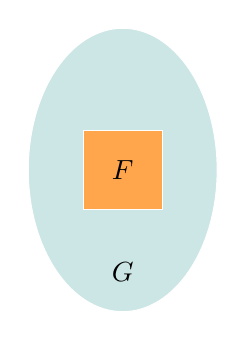
\begin{tikzpicture}
\filldraw[fill=blue!50!green!20, draw=white] (0, 0) ellipse (1.2 and 1.8);
\filldraw[fill=orange!70, draw=white] (-0.5, -0.5) rectangle (0.5, 0.5);
\node at (0, 0) {$F$};
\node at (0, -1.3) {$G$};
\end{tikzpicture}
\hspace{20pt}
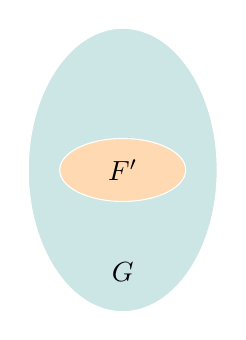
\begin{tikzpicture}
\filldraw[fill=blue!50!green!20, draw=white] (0, 0) ellipse (1.2 and 1.8);
\filldraw[fill=orange!30, draw=white] (0, 0) ellipse (0.8 and 0.4);
\node at (0, 0) {$F'$};
\node at (0, -1.3) {$G$};
\end{tikzpicture}
\hspace{20pt}
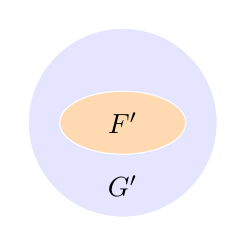
\begin{tikzpicture}
\filldraw[fill=blue!10, draw=white] (0, 0) circle (1.2);
\filldraw[fill=orange!30, draw=white] (0, 0) ellipse (0.8 and 0.4);
\node at (0, 0) {$F'$};
\node at (0, -0.8) {$G'$};
\end{tikzpicture}
\]

或者我们可以首先使用 \hask{beta} 重新包装外部容器,然后应用 \hask{fmap alpha} 重新包装所有内部容器。最终结果是相同的。

\[
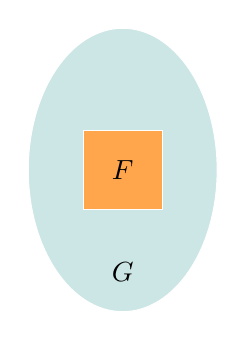
\begin{tikzpicture}
\filldraw[fill=blue!50!green!20, draw=white] (0, 0) ellipse (1.2 and 1.8);
\filldraw[fill=orange!70, draw=white] (-0.5, -0.5) rectangle (0.5, 0.5);
\node at (0, 0) {$F$};
\node at (0, -1.3) {$G$};
\end{tikzpicture}
\hspace{20pt}
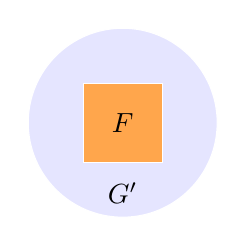
\begin{tikzpicture}
\filldraw[fill=blue!10, draw=white] (0, 0) circle (1.2);
\filldraw[fill=orange!70, draw=white] (-0.5, -0.5) rectangle (0.5, 0.5);
\node at (0, 0) {$F$};
\node at (0, -0.9) {$G'$};
\end{tikzpicture}
\hspace{20pt}
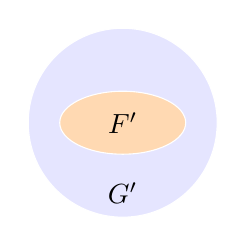
\begin{tikzpicture}
\filldraw[fill=blue!10, draw=white] (0, 0) circle (1.2);
\filldraw[fill=orange!30, draw=white] (0, 0) ellipse (0.8 and 0.4);
\node at (0, 0) {$F'$};
\node at (0, -0.9) {$G'$};
\end{tikzpicture}
\]

\begin{exercise}
实现 \hask{safeHead} 在 \hask{reverse} 之后的水平复合的两个版本。比较它们在不同参数上的作用结果。
\end{exercise}

\begin{exercise}
对 \hask{reverse} 在 \hask{safeHead} 之后的水平复合做同样的操作。
\end{exercise}

\subsection{Whiskering(whiskering)}

在水平组合中,经常会出现其中一个自然变换是恒等变换的情况。对于这种组合,有一种简写表示法。例如,$\beta \circ id_F$ 可以写成 $\beta \circ F$。

由于这种组合的图形特征形状,它被称为“whiskering”。
\[
\begin{tikzcd}[column sep=huge]
\mathcal{C}
 \arrow[r, "F"]
 &
\mathcal{D}
  \arrow[bend left=50]{r}[name=U1, label=above:$G$]{}
  \arrow[bend right=50]{r}[name=D1, label=below:$G'$]{} 
 &
\mathcal{E}
  \arrow[shorten <=10pt,shorten >=10pt,Rightarrow,to path={(U1) -- node[label=left:$\beta$] {} (D1)}]{}
\end{tikzcd}
\]
在分量形式中,我们有:
\[ (\beta \circ F)_x = \beta_{F x} \]

让我们考虑如何将其翻译到 Haskell 中。自然变换是一个多态函数。由于参数化,它对于所有类型都由相同的公式定义。因此,右侧的 whiskering 不会改变公式,而是改变函数签名。

例如,如果这是 \hask{beta} 的声明:
\begin{haskell}
beta :: forall x. G x -> G' x
\end{haskell}
那么它的 whiskered 版本将是:
\begin{haskell}
beta_f :: forall x. G (F x) -> G' (F x)
beta_f = beta
\end{haskell}
由于 Haskell 的类型推断,这种转换是隐式的。当调用多态函数时,我们不需要指定执行自然变换的哪个分量——类型检查器通过查看参数的类型来推断它。

在这种情况下,直觉是我们在重新包装外部容器,同时保持内部容器不变。

类似地,$id_G \circ \alpha$ 可以写成 $G \circ \alpha$。
\[
\begin{tikzcd}[column sep=huge]
\mathcal{D}
  \arrow[bend left=50]{r}[name=U, label=above:$F$]{}
  \arrow[bend right=50]{r}[name=D, label=below:$F'$]{} 
 &
\mathcal{E}
\arrow[r, "G"]
&
\mathcal{F}
  \arrow[shorten <=10pt,shorten >=10pt,Rightarrow,to path={(U) -- node[label=left:$\alpha$] {} (D)}]{}
\end{tikzcd}
\]
在分量形式中:
\[(G \circ \alpha)_x = G (\alpha_x) \]

在 Haskell 中,$\alpha_x$ 通过 $G$ 的提升是使用 \hask{fmap} 完成的,因此给定:
\begin{haskell}
alpha :: forall x. F x -> F' x
\end{haskell}
whiskered 版本将是:
\begin{haskell}
g_alpha :: forall x. G (F x) -> G (F' x)
g_alpha = fmap alpha
\end{haskell}
同样,Haskell 的类型推断引擎会确定使用哪个版本的 \hask{fmap}(在这里,它是 \hask{G} 的 \hask{Functor} 实例中的那个)。

直觉是我们在重新包装内部容器的内容,同时保持外部容器不变。

最后,在许多应用中,自然变换在两侧都被 whiskered:
\[
\begin{tikzcd}[column sep=huge]
\mathcal{C}
 \arrow[r, "F"]
 &
\mathcal{D}
  \arrow[bend left=50]{r}[name=U1, label=above:$G$]{}
  \arrow[bend right=50]{r}[name=D1, label=below:$G'$]{} 
 &
\mathcal{E}
  \arrow[shorten <=10pt,shorten >=10pt,Rightarrow,to path={(U1) -- node[label=left:$\beta$] {} (D1)}]{}
  \arrow[r, "H"]
 &
 \mathcal{F}
\end{tikzcd}
\]
在分量形式中,我们有:
\[ (H \circ \beta \circ F) x = H (\beta_{F x})\]
在 Haskell 中:
\begin{haskell}
h_beta_f :: forall x. H (G (F x)) -> H (G' (F x))
h_beta_f = fmap beta
\end{haskell}

这里的直觉是,我们有一个三层的容器;我们正在重新排列中间的那一层,同时保持外部容器和所有内部容器不变。

\subsection{交换律}

我们可以将垂直复合与水平复合结合起来,如下图所示:
\[
\begin{tikzcd}[column sep=huge]
\mathcal{C}
  \arrow[bend left=60]{rr}[name=U, label=above:$F$]{}
  \arrow[]{rr}[name=M, label={[xshift=15pt, yshift=-5pt]:$G$}]{} 
  \arrow[bend right=60]{rr}[name=D, label=below:$H$]{} 
 &&
\mathcal{D}
  \arrow[bend left=60]{rr}[name=U1, label=above:$F'$]{}
  \arrow[]{rr}[name=M1, label={[xshift=15pt, yshift=-5pt]:$G'$}]{} 
  \arrow[bend right=60]{rr}[name=D1, label=below:$H'$]{} 
&&
\mathcal{E}
  \arrow[shorten <=8pt, shorten >=8pt,Rightarrow, to path={(U) -- node[label=left:$\alpha$] {} (M)}]{}
  \arrow[shorten <=8pt, shorten >=8pt,Rightarrow, to path={(M) -- node[label=left:$\beta$] {} (D)}]{}
  \arrow[shorten <=8pt, shorten >=8pt,Rightarrow, to path={(U1) -- node[label=left:$\alpha'$] {} (M1)}]{}
  \arrow[shorten <=8pt, shorten >=8pt,Rightarrow, to path={(M1) -- node[label=left:$\beta'$] {} (D1)}]{}
\end{tikzcd}
\]
交换律表明复合的顺序无关紧要:我们可以先进行垂直复合再进行水平复合,或者先进行水平复合再进行垂直复合。




\section{重新审视万有构造}

老子曰:大道至简。

我们已经见过和、积、指数、自然数和列表的定义。

定义这些数据类型的传统方法是探究其内部结构。这是集合论的方式:我们观察新集合的元素是如何从旧集合的元素构造出来的。和的元素要么是第一个集合的元素,要么是第二个集合的元素。积的元素是一对元素。依此类推。我们是从工程的角度来看待对象。

在范畴论中,我们采取相反的方法。我们对对象内部是什么或如何实现不感兴趣。我们感兴趣的是对象的目的、如何使用它以及它如何与其他对象交互。我们是从功利的角度来看待对象。

这两种方法各有优势。范畴论的方法出现较晚,因为你需要研究很多例子才能看到清晰的模式。但一旦你看到了这些模式,你就会发现事物之间意想不到的联系,比如和与积的对偶性。

通过对象之间的联系来定义特定对象,需要考虑可能与它们交互的无限多个对象。

“告诉我你与宇宙的关系,我就能告诉你你是谁。”

通过对象在范畴中所有对象的映射出或映射进来定义对象,称为\emph{万有构造}。

为什么自然变换如此重要?因为大多数范畴构造都涉及交换图。如果我们可以将这些图重新表述为自然性方块,我们就在抽象的阶梯上提升了一个层次,并获得了新的有价值的见解。

能够将大量事实压缩成简洁优雅的公式,有助于我们看到新的模式。例如,我们将看到,hom-集之间的自然同构在范畴论中无处不在,并最终引出了伴随的概念。

但首先,我们将更详细地研究几个例子,以理解范畴论的简洁语言。例如,我们将尝试解码以下陈述:两个对象的和或余积由以下自然同构定义:

\[ [\mathbf{2}, \mathcal{C}](D, \Delta_x)  \cong \mathcal{C}(a + b, x) \]

\subsection{选择对象}

即使在范畴论中,像指向对象这样简单的任务也有特殊的解释。我们已经看到,指向集合中的一个元素等价于从单例集合到它的函数的选择。类似地,在范畴中选择一个对象等价于从单对象范畴中选择一个函子。或者,可以使用来自另一个范畴的常函子来完成。

很多时候,我们希望选择一对对象。这也可以通过从两对象的简笔图范畴中选择一个函子来实现。类似地,选择一个箭头等价于从“行走箭头”范畴中选择一个函子,依此类推。

通过明智地选择我们的函子和它们之间的自然变换,我们可以重新表述我们迄今为止见过的所有万有构造。

\subsection{余跨度作为自然变换}

和的定义需要选择两个要相加的对象;以及第三个对象作为映射出的目标。

\[
 \begin{tikzcd}
 a
 \arrow[dr,  bend left, "\text{左}"']
 \arrow[ddr, bend right, "f"']
 && b
 \arrow[dl, bend right, "\text{右}"]
 \arrow[ddl, bend left, "g"]
 \\
&a + b
\arrow[d, dashed, "h"]
\\
& c
 \end{tikzcd}
\]
这个图可以进一步分解为两个更简单的形状,称为\emph{余跨度}:
\[
 \begin{tikzcd}
 a
 \arrow[dr, ""']
 && b
 \arrow[dl, ""]
 \\
 & x
 \end{tikzcd}
\]

要构造一个余跨度,我们首先需要选择一对对象。为此,我们将从一个两对象范畴$\mathbf{2}$开始。我们将其对象称为$1$和$2$。
我们将使用一个函子
\[ D \colon \mathbf{2} \to \mathcal{C}\]
来选择对象$a$和$b$:
\begin{align*}
D\, 1 &= a \\
D\, 2 &= b 
\end{align*}
($D$代表“图”,因为这两个对象在$\mathcal{C}$中形成了一个非常简单的图,由两个点组成。)

我们将使用常函子
\[ \Delta_x \colon \mathbf{2} \to \mathcal{C} \]
来选择对象$x$。这个函子将$1$和$2$都映射到$x$(并将两个恒等箭头映射到$id_x$)。

由于这两个函子都从$\mathbf{2}$到$\mathcal{C}$,我们可以定义它们之间的自然变换$\alpha$。在这种情况下,它只是一对箭头:
\begin{align*}
\alpha_1 \colon D \, 1 \to \Delta_x 1 \\
\alpha_2 \colon D \, 2 \to \Delta_x 2
\end{align*}
这些正是余跨度中的两个箭头。

$\alpha$的自然性条件是平凡的,因为$\mathbf{2}$中没有箭头(除了恒等箭头)。

可能有许多余跨度共享相同的三个对象——这意味着:可能有许多自然变换在函子$D$和$\Delta_x$之间。这些自然变换形成了函子范畴$[\mathbf{2}, \mathcal{C}]$中的一个hom-集,即:
\[ [\mathbf{2}, \mathcal{C}](D, \Delta_x) \]

\subsection{余跨度的函子性}

让我们考虑当我们在余跨度中开始变化对象$x$时会发生什么。我们有一个映射$F$,它将$x$映射到$x$上的余跨度集:
\[ F x = [\mathbf{2}, \mathcal{C}](D, \Delta_x) \]
这个映射在$x$上是函子性的。

要看到这一点,考虑一个箭头$m \colon x \to y$。这个箭头的提升是两个自然变换集之间的映射:
\[ [\mathbf{2}, \mathcal{C}](D, \Delta_x) \to [\mathbf{2}, \mathcal{C}](D, \Delta_{y}) \] 
 
这可能看起来非常抽象,直到你记住自然变换有分量,而这些分量只是常规箭头。左边的一个元素是一个自然变换:
\[ \mu \colon D \to \Delta_x \]
它有两个分量,对应于$\mathbf{2}$中的两个对象。例如,我们有
\[ \mu_1 \colon D \, 1 \to \Delta_x 1 \]
或者,使用$D$和$\Delta$的定义:
\[ \mu_1 \colon a \to x \]
这只是我们余跨度的左腿。

类似地,右边的一个元素是一个自然变换:
\[ \nu \colon D \to \Delta_{y} \]
它在$1$处的分量是一个箭头
\[ \nu_1 \colon a \to y \]
我们可以通过将$\mu_1$与$m \colon x \to y$后复合来从$\mu_1$得到$\nu_1$。因此,$m$的提升是分量逐个分量的后复合$(m \circ -)$:
\begin{align*}
\nu_1 = m \circ \mu_1 \\
\nu_2 = m \circ \mu_2 \\
\end{align*}

\subsection{和作为万有余跨度}

在你可以构建在$a$和$b$上的所有余跨度中,具有我们称为$\text{左}$和$\text{右}$的箭头汇聚在$a + b$上的那个非常特殊。从它到任何其他余跨度都有一个唯一的映射——一个使两个三角形交换的映射。
\[
 \begin{tikzcd}
 a
 \arrow[dr,  bend left, "\text{左}"']
 \arrow[ddr, bend right, "f"']
 && b
 \arrow[dl, bend right, "\text{右}"]
 \arrow[ddl, bend left, "g"]
 \\
&a + b
\arrow[d, dashed, "h"]
\\
& x
 \end{tikzcd}
\]

我们现在可以将这个条件转化为关于自然变换和hom-集的陈述。箭头$h$是hom-集
\[ \mathcal{C}(a + b, x)\]
中的一个元素。$x$上的余跨度是一个自然变换,即函子范畴中的hom-集的一个元素:
\[ [\mathbf{2}, \mathcal{C}](D, \Delta_x) \]

两者都是各自范畴中的hom-集。两者都只是集合,即范畴$\mathbf{Set}$中的对象。这个范畴在函子范畴$[\mathbf{2}, \mathcal{C}]$和“常规”范畴$\mathcal{C}$之间架起了一座桥梁,尽管在概念上它们似乎处于非常不同的抽象层次。

借用西格蒙德·弗洛伊德的话,“有时候,集合就是集合。”

我们的万有构造是集合的双射或同构:
\[ [\mathbf{2}, \mathcal{C}](D, \Delta_x)  \cong \mathcal{C}(a + b, x) \]

此外,如果我们变化对象$x$,这两边表现得像从$\mathcal{C}$到$\mathbf{Set}$的函子。因此,询问这个函子映射是否是自然同构是有意义的。

事实上,可以证明这个同构的自然性条件转化为和定义中三角形的交换条件。因此,和的定义可以用一个单一的方程来替代。

\subsection{积作为万有跨度}

关于积的万有构造,可以提出类似的论点。再次,我们从简笔图范畴$\mathbf{2}$和函子$D$开始。但这次我们使用一个自然变换,方向相反
\[ \alpha \colon \Delta_x \to D \]
这样的自然变换是一对箭头,形成一个\emph{跨度}:
\[
 \begin{tikzcd}
 &x
 \arrow[dl, "f"']
 \arrow[dr, "g"]
 \\
 a
 && b
  \end{tikzcd}
\]
这些自然变换共同形成了函子范畴中的一个hom-集:
\[[\mathbf{2}, \mathcal{C}](\Delta_x, D) \]

这个hom-集的每个元素都与一个唯一的映射$h$到积$a \times b$一一对应。这样的映射是hom-集$\mathcal{C}(x, a \times b)$的一个成员。这种对应关系表示为同构:
\[ [\mathbf{2}, \mathcal{C}](\Delta_x, D)  \cong \mathcal{C}(x, a \times b) \]
可以证明,这个同构的自然性保证了图中三角形的交换:
\[
 \begin{tikzcd}
 & x
\arrow[d, dashed, "h"]
 \arrow[ddl, bend right, "f = \alpha_1"']
 \arrow[ddr, bend left, "g = \alpha_2"]
\\
&a \times b
 \arrow[dl,  "\text{fst}"]
  \arrow[dr,   "\text{snd}"']
\\
a = D\, 1 && b = D \, 2
 \end{tikzcd}
\]

\subsection{指数}

指数或函数对象由以下交换图定义:
\[
 \begin{tikzcd}
 x \times a
 \arrow[d, dashed, "h \times id_a"']
 \arrow[rd, "f"]
 \\
 b^a \times a
 \arrow[r, "\varepsilon_{a b}"']
& b
 \end{tikzcd}
\]
这里,$f$是hom-集$\mathcal{C}(x \times a, b)$的一个元素,$h$是$\mathcal{C}(x, b^a)$的一个元素。

这些集合之间的同构,在$x$上是自然的,定义了指数对象。
\[\mathcal{C}(x \times a, b) \cong \mathcal{C}(x, b^a)\]

上图中的$f$是左边的一个元素,$h$是右边对应的元素。变换$\alpha_x$(它也依赖于$a$和$b$)将$f$映射到$h$。
\[ \alpha_x \colon \mathcal{C}(x \times a, b) \to \mathcal{C}(x, b^a) \]
在Haskell中,我们称之为\hask{curry}。它的逆$\alpha^{-1}$被称为\hask{uncurry}。

与前面的例子不同,这里两个hom-集都在同一个范畴中,因此更容易详细分析同构。特别是,我们希望看到交换条件:
\[  f = \varepsilon_{a b} \circ (h \times id_a) \]
是如何从自然性中产生的。

标准的Yoneda技巧是对$x$进行替换,将其中一个hom-集简化为自hom-集,即源与目标相同的hom-集。这将允许我们选择该hom-集的一个规范元素,即恒等箭头。

在我们的情况下,将$b^a$替换为$x$将允许我们选择$h = id_{(b^a)}$。
\[
 \begin{tikzcd}
 b^a \times a
 \arrow[d, dashed, "id_{(b^a)} \times id_a"']
 \arrow[rd, "f"]
 \\
 b^a \times a
 \arrow[r, "\varepsilon_{a b}"']
& b
 \end{tikzcd}
\]
在这种情况下,交换条件告诉我们$f = \varepsilon_{a b}$。换句话说,我们得到了$\varepsilon_{a b}$的公式,用$\alpha$表示:
\[ \varepsilon_{a b} = \alpha_{x}^{-1} (id_{x}) \]
其中$x$等于$b^a$。

由于我们认识到$\alpha^{-1}$是\hask{uncurry},而$\varepsilon$是函数应用,我们可以在Haskell中将其写为:
\begin{haskell}
apply :: (a -> b, a) -> b
apply = uncurry id
\end{haskell}
这可能一开始令人惊讶,直到你意识到\hask{(a->b,a)->b}的柯里化导致\hask{(a->b)->(a->b)}。

我们还可以将主同构的两边编码为Haskell函子:
\begin{haskell}
data LeftFunctor  a b x = LF ((x, a) -> b)
\end{haskell}
\begin{haskell}
data RightFunctor a b x = RF (x -> (a -> b))
\end{haskell}
它们在类型变量\hask{x}中都是逆变函子。
\begin{haskell}
instance Contravariant (LeftFunctor a b) where
  contramap g (LF f) = LF (f . bimap g id)
\end{haskell}
这表示$g \colon x \to y$的提升由以下前复合给出:
\[ \mathcal{C}(y \times a, b) \xrightarrow{(- \circ (g \times id_a)) }  \mathcal{C}(x \times a, b)\]

类似地:
\begin{haskell}
instance Contravariant (RightFunctor a b) where
  contramap g (RF h) = RF (h . g)
\end{haskell}
翻译为:
\[  \mathcal{C}(y, b^a) \xrightarrow{ (- \circ g) } \mathcal{C}(x, b^a) \]

自然变换$\alpha$只是\hask{curry}的薄封装;它的逆是\hask{uncurry}:

\begin{haskell}
alpha :: forall a b x. LeftFunctor a b x -> RightFunctor a b x
alpha (LF f) = RF (curry f)
\end{haskell}

\begin{haskell}
alpha_1 :: forall a b x. RightFunctor a b x -> LeftFunctor a b x
alpha_1 (RF h) = LF (uncurry h)
\end{haskell}

使用$g \colon x \to y$的提升的两个公式,这里是自然性方块:

\[
 \begin{tikzcd}
 \mathcal{C}(y \times a, b)
 \arrow[rr, "(- \circ (g \times id_a))"]
 \arrow[d,  "\alpha_y"]
& &
\mathcal{C}(x \times a, b)
  \arrow[d, "\alpha_x"]
 \\
 \mathcal{C}(y, b^a)
 \arrow[rr, "(- \circ g)"]
& &
\mathcal{C}(x, b^a)
 \end{tikzcd}
\]

现在让我们对其应用Yoneda技巧,并将$y$替换为$b^a$。这也允许我们将$g$——现在从$x$到$b^a$——替换为$h$。

\[
 \begin{tikzcd}
 \mathcal{C}(b^a \times a, b)
 \arrow[rr, "(- \circ (h \times id_a))"]
 \arrow[d,  "\alpha_{(b^a)}"]
& &
\mathcal{C}(x \times a, b)
  \arrow[d,  "\alpha_x"]
 \\
 \mathcal{C}(b^a, b^a)
 \arrow[rr, "(- \circ h)"]
& &
\mathcal{C}(x, b^a)
 \end{tikzcd}
\]

我们知道hom-集$\mathcal{C}(b^a, b^a)$至少包含恒等箭头,因此我们可以在左下角选择元素$id_{(b^a)}$。

反转左边的箭头,我们知道$\alpha^{-1}$作用于恒等产生$\varepsilon_{a b}$在左上角(这是\hask{uncurry id}技巧)。

$h$的前复合作用于恒等产生$h$在右下角。

$\alpha^{-1}$作用于$h$产生$f$在右上角。

\[
 \begin{tikzcd}[
  every arrow/.style={draw,mapsto}
]
 \varepsilon_{a b}
 \arrow[rr, "(- \circ (h \times id_a))"]
& &
f
 \\
 id_{(b^a)}
 \arrow[u, "\alpha^{-1}"]
 \arrow[rr, "(- \circ h)"]
& &
h
\arrow[u, "\alpha^{-1}"']
 \end{tikzcd}
\]
($\mapsto$箭头表示函数对集合元素的作用。)

因此,在左下角选择$id_{(b^a)}$固定了其他三个角。特别是,我们可以看到上箭头应用于$\varepsilon_{a b}$产生$f$,这正是我们想要推导的交换条件:
\[ \varepsilon_{a b} \circ (h \times id_a) = f \]

\section{极限与余极限}

在前一节中,我们使用自然变换定义了和与积。这些变换是在由非常简单的棒图范畴 $\mathbf{2}$ 定义的图之间进行的,其中一个函子是常函子。

没有什么能阻止我们用更复杂的范畴替换 $\mathbf{2}$。例如,我们可以尝试在对象之间具有非平凡箭头的范畴,或者具有无限多个对象的范畴。

围绕这些构造有一整套词汇。

我们使用范畴 $\mathbf{2}$ 中的对象来索引范畴 $\mathcal{C}$ 中的对象。我们可以用任意的索引范畴 $\cat J$ 替换 $\mathbf{2}$。$\mathcal{C}$ 中的图仍然定义为函子 $D \colon \cat J \to \mathcal{C}$。它选择 $\mathcal{C}$ 中的对象,但也选择它们之间的箭头。

作为第二个函子,我们仍然使用常函子 $\Delta_x \colon \cat J \to \mathcal{C}$。

自然变换,即 hom-集
\[ [\cat J, \mathcal{C}](\Delta_x, D)  \]
的元素,现在称为一个\emph{锥}。它的对偶,即
\[ [\cat J, \mathcal{C}](D, \Delta_x)  \]
的元素,称为一个\emph{余锥}。它们分别推广了跨度和余跨度。

在图中,锥和余锥看起来像这样:
\[
 \begin{tikzcd}
  & x
\arrow[ddr, "g"]
 \arrow[ddl, "f"']
 \arrow[ddd, "h"]
 \\
\\
D 1 
\arrow[rr, red]
\arrow[rd, red]
&& D 2
\arrow[dl, red]
\\
& D 3
 \end{tikzcd}
 \qquad
\begin{tikzcd}
 D 1
 \arrow[rr, red]
 \arrow[dr, red]
 \arrow[dddr, "f"']
 && D 2
\arrow[dl, red]
 \arrow[dddl, "g"]
 \\
 & D 3
 \arrow[dd, "h"]
 \\
 \\
 & x
 \end{tikzcd}
 \]

由于索引范畴现在可能包含箭头,这些图的自然性条件不再平凡。常函子 $\Delta_x$ 将所有顶点收缩为一个,因此自然性方块收缩为三角形。自然性意味着所有以 $x$ 为顶点的三角形现在必须交换。

如果存在,通用锥称为图 $D$ 的\emph{极限},并记为 $\text{Lim}D$。通用性意味着它满足以下同构,对于 $x$ 是自然的:
\[ [\cat J, \mathcal{C}](\Delta_x, D)  \cong \mathcal{C}(x, \text{Lim}D) \]
对于每个以 $x$ 为顶点的锥,存在一个从 $x$ 到极限 $ \text{Lim}D$ 的唯一映射。

$\Set$ 值函子的极限有一个特别简单的特征。它是一组以单例集为顶点的锥。实际上,极限的元素,即从单例集到它的函数,与这些锥一一对应:
\[ [\cat J, \mathcal{C}](\Delta_1, D)  \cong \mathcal{C}(1, \text{Lim}D) \]

对偶地,通用余锥称为\emph{余极限},并由以下自然同构描述:
\[ [\cat J, \mathcal{C}](D, \Delta_x)  \cong \mathcal{C}( \text{Colim}D, x) \]

我们现在可以说,积是来自索引范畴 $\mathbf{2}$ 的图的极限(和是余极限)。

极限和余极限提炼了模式的本质。

极限,如积,由其映射入属性定义。余极限,如和,由其映射出属性定义。

有许多有趣的极限和余极限,我们将在讨论代数和余代数时看到一些。

\begin{exercise}
证明\index{行走箭头,极限}“行走箭头”范畴的极限,即具有连接两个对象的箭头的两对象范畴,具有与图中第一个对象相同的元素(“元素”是从终端对象出发的箭头)。
\end{exercise}

\subsection{等化子}

许多高中数学涉及学习如何解方程或方程组。方程将两种不同方式产生的结果等同起来。如果我们允许减去某些东西,我们通常将所有东西移到一边,并将问题简化为计算某个表达式的零点。在几何中,同样的思想表示为两个几何对象的交集。

在范畴论中,所有这些模式都体现在一个称为等化子的单一构造中。等化子是一个图的极限,其模式由具有两个平行箭头的棒图范畴给出:
\[
\begin{tikzcd}
i \arrow[r, shift left=0.75ex]
  \arrow[r, shift right=0.75ex]
&
j
\end{tikzcd}
\]
这两个箭头表示两种产生某物的方式。

从这个范畴的函子选择目标范畴中的一对对象和一对态射。这个图的极限体现了两个结果的交集。它是一个对象 $e$ 和两个箭头 $p \colon e \to a$ 和 $p' \colon e \to b$。
\[
\begin{tikzcd}
& e
\arrow[dl, "p"']
\arrow[dr, gray, "p'"]
\\
a 
\arrow[rr, red, shift left=.75ex, "f"]
\arrow[rr, red, shift right=.75ex, "g"']
&&
b
\end{tikzcd}
\]
我们有两个交换条件:
\begin{align*}
p' &= f \circ p \\
p' &= g \circ p
\end{align*}
这意味着 $p'$ 由其中一个方程完全确定,而另一个方程转化为约束:
\[ f \circ p = g \circ p \]
由于等化子是极限,它是通用的这样一对,如图所示:
\[
\begin{tikzcd}
x
\arrow[d, dashed, "h"']
\arrow[dr, ""]
\\
e
\arrow[r, "p"']
&
a \arrow[r, red, shift left=0.75ex, "f"]
  \arrow[r, red, shift right=0.75ex, "g"']
&
b
\end{tikzcd}
\]

为了发展对等化子的直觉,考虑它在集合中的工作方式是有益的。通常,技巧是将 $x$ 替换为单例集 $1$:
\[
\begin{tikzcd}
1
\arrow[d, dashed, "e"']
\arrow[dr, "a"]
\\
E
\arrow[r, "p"']
&
A \arrow[r, red, shift left=0.75ex, "f"]
  \arrow[r, red, shift right=0.75ex, "g"']
&
B
\end{tikzcd}
\]
在这种情况下,$a$ 是 $A$ 的一个元素,使得 $f a = g a$。这只是说 $a$ 是由一对函数定义的方程的解。通用性意味着存在一个唯一的元素 $e$ 属于 $E$,使得 $p \circ e = a$。换句话说,$E$ 的元素与方程组的解一一对应。

\subsection{余等化子}

与等同或交集对偶的概念是什么?它是发现共性并将事物组织到桶中的过程。例如,我们可以将整数分配到偶数和奇数桶中。在范畴论中,这种桶化过程由余等化子描述。

余等化子是用于定义等化子的相同图的余极限:
\[
\begin{tikzcd}
a 
\arrow[rr, red, shift left=.75ex, "f"]
\arrow[rr, red, shift right=.75ex, "g"']
\arrow[rd, gray, "q'"']
&&
b
\arrow[ld, "q"]
\\
& c
\end{tikzcd}
\]
这一次,箭头 $q'$ 由 $q$ 完全确定;并且 $q$ 必须满足方程:
\[ q \circ f = q \circ g \]

再次,我们可以通过考虑两个函数在集合上的余等化子来获得一些直觉。
\[
\begin{tikzcd}
A
\arrow[r, red, shift left=.75ex, "f"]
\arrow[r, red, shift right=.75ex, "g"']
&
B
\arrow[r, "q"]
& C
\end{tikzcd}
\]
一个 $x \in A$ 被映射到 $B$ 中的两个元素 $f x$ 和 $g x$,但然后 $q$ 必须将它们映射回 $C$ 中的一个元素。这个元素代表桶。

通用性意味着 $C$ 是 $B$ 的一个副本,其中从同一个 $x$ 产生的元素已被识别。

考虑一个例子,其中 $A$ 是一对整数的集合 \hask{(m, n)},使得它们要么都是偶数,要么都是奇数。我们想要余等化两个函数,即两个投影 \hask{(fst, snd)}。等化子集 $C$ 将有两个元素对应于两个桶。我们将它表示为 \hask{Bool}。等化函数 \hask{q} 选择桶:
\begin{haskell}
q :: Int -> Bool
q n = n `mod` 2 == 0 
\end{haskell}
任何函数 \hask{q'} 如果不能区分我们对的组件,并且只对它们的奇偶性敏感:
\[ q' \circ \mathvar{fst} = q' \circ \mathvar{snd} \]
可以通过函数 \hask{h} 唯一地分解:
\begin{haskell}
h :: (Int -> a) -> Bool -> a
h q' True  = q' 0
h q' False = q' 1
\end{haskell}

\[
\begin{tikzcd}
(\text{Int}, \text{Int})
\arrow[r, red, shift left=.75ex, "\text{fst}"]
\arrow[r, red, shift right=.75ex, "\text{snd}"']
&
\text{Int}
\arrow[r, "q"]
\arrow[rd, "q'"']
& \text{Bool}
\arrow[d, dashed, "h"]
\\
&& A
\end{tikzcd}
\]

\begin{exercise}
运行一些测试,显示分解 $(h\, q') \circ q$ 给出与 \hask{q'} 相同的结果,其中 \hask{q'} 由以下定义给出:
\begin{haskell}
import Data.Bits

q' :: Int -> Bool
q' x = testBit x 0
\end{haskell}

\end{exercise}

\subsection{终端对象的存在性}

老子说:伟大的行为由小行为组成。

到目前为止,我们一直在研究小图的极限,即来自简单棒图范畴的函子。然而,没有什么能阻止我们定义极限和余极限,其中模式被取为无限范畴。但无限性有等级之分。当范畴中的对象形成一个真集时,我们称这样的范畴为\index{小范畴}\emph{小}范畴。不幸的是,最基本的例子,集合的范畴 $\Set$,不是小范畴。我们知道没有所有集合的集合。$\Set$ 是一个\index{大范畴}\emph{大}范畴。但至少 $\Set$ 中的所有 hom 集都是集合。我们说 $\Set$ 是\index{局部小范畴}\emph{局部小}的。在接下来的内容中,我们将始终处理局部小范畴。

小极限是小图的极限,即来自对象和态射形成集合的范畴的函子。所有小极限存在的范畴称为小完备的,或简称为\emph{完备}的。特别是,在这样的范畴中,任意\emph{集}的对象的积存在。你也可以等化两个对象之间的任意集箭头。如果这样的范畴是局部小的,这意味着所有等化子都存在。

相反,一个(小)余完备范畴具有所有小余极限。特别是,这样的范畴具有所有小余积和余等化子。

范畴 $\Set$ 既是完备的又是余完备的。

在余完备的局部小范畴中,存在终端对象的一个简单标准:存在弱终端集就足够了。

\index{弱终端对象}\emph{弱终端}对象,就像终端对象一样,有来自任何对象的箭头;只是这样的箭头不一定是唯一的。

\index{弱终端集}\emph{弱终端集}是由集合 $I$ 索引的对象族 $t_i$,使得对于 $\cat C$ 中的任何对象 $c$,存在一个 $i$ 和一个箭头 $c \to t_i$。这样的集也称为\index{解集}\emph{解集}。

\[
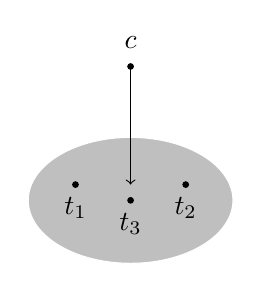
\begin{tikzpicture}
        \filldraw (0, 1.5) circle (1pt);
        \node at (0, 1.8) {$c$};
        
\filldraw[fill=gray!50, draw=white] (0, -0.2) ellipse (1.3 and 0.8);
        \filldraw (-0.7, 0) circle (1pt);
        \node at (-0.7, -0.3) {$t_1$};
        \filldraw (0.7, 0) circle (1pt);
        \node at (0.7, -0.3) {$t_2$};
        \filldraw (0, -0.2) circle (1pt);
        \node at (0, -0.5) {$t_3$};
        
    	\draw[->] (0, 1.5) -- (0, 0);
\end{tikzpicture}
\]

在余完备范畴中,我们总是可以构造一个余积 $\coprod_{i \in I} t_i$。这个余积是一个弱终端对象,因为从每个 $c$ 都有一个箭头指向它。这个箭头是从某个 $t_i$ 的箭头后跟注入 $\iota_i \colon t_i \to \coprod_{j \in I} t_j$ 的复合。

给定一个弱终端对象,我们可以构造(强)终端对象。我们首先定义 $\cat C$ 的一个子范畴 $\cat T$,其对象是 $t_i$。$\cat T$ 中的态射是 $\cat C$ 中所有在 $\cat T$ 的对象之间进行的态射。这称为 $\cat C$ 的\index{全子范畴}\emph{全}子范畴。根据我们的构造,$\cat T$ 是小的。

有一个明显的包含函子 $F$ 将 $\cat T$ 嵌入 $\cat C$。这个函子在 $\cat C$ 中定义了一个小图。事实证明,这个图的余极限是 $\cat C$ 中的终端对象。

对偶地,类似的构造可以用于将初始对象定义为弱初始集的极限。

解集的这个属性将在证明 Freyd 的伴随函子定理时派上用场。

\section{米田引理 (Yoneda Lemma)}

从某个范畴 $\mathcal{C}$ 到集合范畴的函子可以被视为该范畴在 $\mathbf{Set}$ 中的模型。一般来说,建模是一个有损的过程:它会丢弃一些信息。一个常值 $\Set$-值函子是一个极端的例子:它将整个范畴映射到一个单一的集合及其恒等函数。

同态函子 (hom-functor) 从某个视角生成该范畴的模型。例如,函子 $\mathcal{C}(a, -)$ 提供了从 $a$ 的视角看到的 $\mathcal{C}$ 的全景图。它将所有从 $a$ 出发的箭头组织成整齐的包,这些包通过箭头之间的图像连接起来,所有这些都符合源范畴的原始结构。

\[
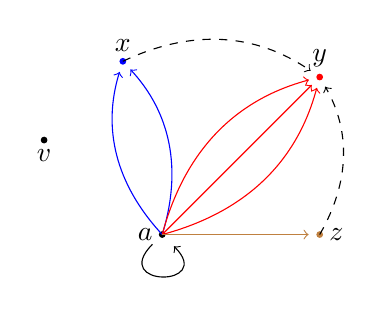
\begin{tikzpicture}
\def\ax{0}
\def\ay{0.5}
\def\xx{-0.5}
\def\xy{2.7}
\def\yx{2}
\def\yy{2.5}
\def\zx{2}
\def\zy{0.5}
\def\vx{-1.5}
\def\vy{1.7}
\filldraw[black] (\ax, \ay) circle (1 pt);
\node (a) at (\ax, \ay) {};
\node[left] at (\ax, \ay) {$a$};
\filldraw[blue] (\xx, \xy) circle (1 pt);
\node[above] at (\xx, \xy) {$x$};
\filldraw[red] (\yx, \yy) circle (1 pt);
\node[above] at (\yx, \yy) {$y$};
\filldraw[brown] (\zx, \zy) circle (1 pt);
\node[right] at (\zx, \zy) {$z$};
\filldraw[black] (\vx, \vy) circle (1 pt);
\node[below] at (\vx, \vy) {$v$};

\draw [->] (a) edge[out=225, in=315, loop] (a);

\draw[dashed] (\xx, \xy) edge[->, bend left, shorten > = 4 pt] (\yx, \yy);
\draw[dashed] (\zx, \zy) edge[->, bend right, shorten > = 4 pt] (\yx, \yy);

\draw[blue] (\ax, \ay) edge[->, bend left, shorten > = 4 pt] (\xx, \xy);
\draw[blue] (\ax, \ay) edge[->, bend right, shorten > = 4 pt] (\xx, \xy);

\draw[red] (\ax, \ay) edge[->, bend left, shorten > = 4 pt] (\yx, \yy);
\draw[red] (\ax, \ay) edge[->, bend right, shorten > = 4 pt] (\yx, \yy);
\draw[red] (\ax, \ay) edge[->, shorten > = 4 pt] (\yx, \yy);

\draw[brown] (\ax, \ay) edge[->, shorten > = 4 pt] (\zx, \zy);
\end{tikzpicture}
\hspace{80pt}
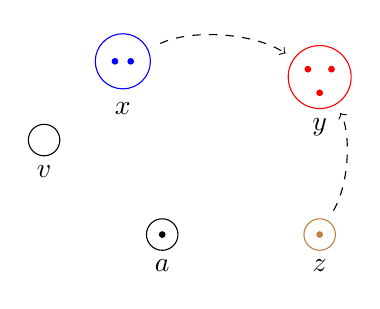
\begin{tikzpicture}
\def\ax{0}
\def\ay{0.5}
\def\xx{-0.5}
\def\xy{2.7}
\def\yx{2}
\def\yy{2.5}
\def\zx{2}
\def\zy{0.5}
\def\vx{-1.5}
\def\vy{1.7}
\def\sx{0.7}
\def\sy{1.6}

\node at (\sx, \sy) {$\Set$};

\draw[black] (\vx, \vy) circle (0.2);
\node[below] at (\vx, \vy - 0.2) {$v$};

\draw[black] (\ax, \ay) circle (0.2);
\filldraw[black] (\ax, \ay) circle (1 pt);
\node[below] at (\ax, \ay-0.2) {$a$};

\draw[blue] (\xx, \xy) circle (0.35);
\filldraw[blue] (\xx - 0.1, \xy) circle (1 pt);
\filldraw[blue] (\xx + 0.1, \xy) circle (1 pt);
\node[above] at (\xx, \xy - 0.8) {$x$};

\draw[red] (\yx, \yy) circle (0.4);
\filldraw[red] (\yx-0.15, \yy+0.1) circle (1 pt);
\filldraw[red] (\yx+0.15, \yy+0.1) circle (1 pt);
\filldraw[red] (\yx, \yy-0.2) circle (1 pt);
\node[below] at (\yx, \yy - 0.4) {$y$};

\draw[brown] (\zx, \zy) circle (0.2);
\filldraw[brown] (\zx, \zy) circle (1 pt);
\node[below] at (\zx, \zy - 0.2) {$z$};

\draw[dashed] (\xx, \xy) edge[->, bend left, shorten > = 15, shorten < = 15] (\yx, \yy);
\draw[dashed] (\zx, \zy) edge[->, bend right, shorten > = 15, shorten < = 10] (\yx, \yy);

\end{tikzpicture}
\]

有些视角比其他视角更好。例如,从初始对象 (initial object) 的视角看,视图相当稀疏。每个对象 $x$ 都被映射到一个单例集 $\cat C(0, x)$,对应于唯一的映射 $0 \to x$。

从终止对象 (terminal object) 的视角看则更有趣:它将所有对象映射到它们的(全局)元素集 $\cat C(1, x)$。

米田引理可以被视为范畴论中最深刻的陈述之一,或者是最平凡的陈述之一。让我们从深刻的版本开始。

考虑 $\mathcal{C}$ 在 $\mathbf{Set}$ 中的两个模型。第一个由同态函子 $\mathcal{C}(a, -)$ 给出。这是从 $a$ 的视角看到的 $\mathcal{C}$ 的全景图,非常详细。第二个由某个任意函子 $F \colon \mathcal{C} \to \mathbf{Set}$ 给出。它们之间的任何自然变换 (natural transformation) 都将一个模型嵌入到另一个模型中。事实证明,所有这样的自然变换的集合完全由集合 $F a$ 决定。

由于自然变换的集合是函子范畴 $[\mathcal{C}, \mathbf{Set}]$ 中的同态集,米田引理的形式化陈述如下:

\[ [\mathcal{C}, \mathbf{Set}]( \mathcal{C}(a, -), F) \cong F a \]
此外,这个同构在 $a$ 和 $F$ 中都是自然的。

之所以这能成立,是因为该定理中涉及的所有映射都受到保持范畴 $\mathcal{C}$ 结构及其模型结构的约束。特别是,自然性条件对自然变换的组成部分从一个点传播到另一个点的方式施加了大量的约束。

米田引理的证明从一个单一的恒等箭头开始,并让自然性将其传播到整个范畴。

以下是证明的概要。它由两部分组成:首先,给定一个自然变换,我们构造 $F a$ 的一个元素。其次,给定 $F a$ 的一个元素,我们构造相应的自然变换。

首先,让我们在米田引理的左侧选择一个任意元素:一个自然变换 $\alpha$。它在 $x$ 处的分量是一个函数:
\[ \alpha_x \colon \mathcal{C}(a, x) \to F x \]
我们现在可以应用米田技巧:将 $a$ 替换为 $x$:
\[ \alpha_a \colon \mathcal{C}(a, a) \to F a \]
然后选择恒等 $id_a$ 作为 $\mathcal{C}(a, a)$ 的规范元素。结果是集合 $F a$ 中的一个元素 $\alpha_a (id_a)$。这定义了一个从自然变换到集合 $F a$ 元素的映射。

现在反过来。给定集合 $F a$ 的一个元素 $p$,我们想要构造一个自然变换 $\alpha$。首先,我们将 $p$ 分配为 $\alpha_a$ 在 $id_a \in \cat C(a, a)$ 上的作用。

\[
\begin{tikzpicture}
\def\ax{0}
\def\ay{0.5}
\def\xx{-0.5}
\def\xy{3.7}
\filldraw[black] (\ax, \ay) circle (1 pt);
\node (a) at (\ax, \ay) {};
\node[left] at (\ax, \ay) {$a$};
\filldraw[blue] (\xx, \xy) circle (1 pt);
\node[above] at (\xx, \xy) {$x$};

\draw [->] (a) edge[out=225, in=315, loop] (a);
\node[right] at (\ax + 0.3, \ay - 0.35) {$id_a$};

\draw[blue] (\ax, \ay) edge[->, "$h$", bend right, shorten > = 4 pt] (\xx, \xy);

\end{tikzpicture}
\hspace{80pt}
\begin{tikzpicture}

\def\ax{0}
\def\ay{0.5}
\def\xx{-0.5}
\def\xy{3.7}

\def\fax{3}
\def\fay{0.5}
\def\fxx{3 - 0.5}
\def\fxy{3.7}

\def\px{\fax - 0.3}
\def\hx{\xx + 0.35}
% C(a,a)
\draw[black] (\ax, \ay) circle (0.2);
\filldraw[black] (\ax, \ay) circle (1 pt);
\node[below] at (\ax, \ay-0.2) {$\cat C (a, a)$};
% C(a,x)
\draw[black] (\xx, \xy) ellipse (0.7 and 0.4);

\filldraw[blue] (\xx + 0.35, \xy) circle (1 pt);
\node[left, blue] at (\hx, \xy) {$h$};

\node[above] at (\xx, \xy - 1.1) {$\cat C (a, x)$};
\draw[dashed] (\hx, \xy) edge[->, "$\alpha_x$", shorten > = 4 pt] (\fxx, \fxy);

% F a
\draw[red] (\fax, \fay) ellipse (0.7 and 0.4);
\filldraw[red] (\px, \fay) circle (1 pt);
\node[right, red] at (\px, \fay) {$p$};
\node[right, red] at (\fax + 0.7, \fay) {$F a$};
\draw[dashed] (\ax, \ay) edge[->, "$\alpha_a$", shorten > = 3 pt] (\px, \fay);
% F x
\draw[red] (\fxx, \fxy) circle (0.4);
\filldraw[red] (\fxx, \fxy) circle (1 pt);
\node[right, red] at (\fxx + 0.35, \fxy) {$F x$};

\draw[blue] (\px, \fay) edge[->, "$F h$", bend right, shorten > = 12, shorten < = 12] (\fxx, \fxy);

\end{tikzpicture}
\]

现在让我们取一个任意对象 $x$ 和 $\cat C(a, x)$ 的一个任意元素。后者是一个箭头 $h \colon a \to x$。我们的自然变换必须将其映射到 $F x$ 的一个元素。我们可以通过使用 $F$ 提升箭头 $h$ 来实现这一点。我们得到一个函数:
\[F h \colon F a \to F x \]
我们可以将这个函数应用于 $p$ 并得到 $F x$ 的一个元素。我们将这个元素作为 $\alpha_x$ 在 $h$ 上的作用:
\[ \alpha_x h = (F h) p \]

米田引理中的同构在 $a$ 和 $F$ 中都是自然的。后者意味着你可以通过在函子范畴中应用一个箭头(即自然变换)从函子 $F$ “移动”到另一个函子 $G$。这是在抽象层次上的一个巨大飞跃,但所有关于函子性和自然性的定义在函子范畴中同样适用,其中对象是函子,箭头是自然变换。

\begin{exercise}
当 $F a$ 为空时,填补证明中的空白。
\end{exercise}
\begin{exercise}
证明上述定义的映射
\[ \mathcal{C}(a, x) \to F x\]
是一个自然变换。提示:使用某个 $f \colon x \to y$ 来变化 $x$。
\end{exercise}
\begin{exercise}
证明 $\alpha_x$ 的公式可以从 $\alpha_a (id_a) = p$ 和自然性条件推导出来。提示:同态函子 $\cat C(a, h)$ 对 $h$ 的提升由后复合给出。
\end{exercise}

\subsection{编程中的米田引理}

现在来看平凡的部分:米田引理的证明直接翻译为 Haskell 代码。我们从同态函子 \hask{a->x} 和某个函子 \hask{f} 之间的自然变换类型开始,并证明它等价于 \hask{f} 作用于 \hask{a} 的类型。
\begin{haskell}
forall x. (a -> x) -> f x.   -- 同构于 (f a)
\end{haskell}
我们使用标准的米田技巧生成类型 \hask{(f a)} 的值
\begin{haskell}
yoneda :: Functor f => (forall x. (a -> x) -> f x) -> f a
yoneda g = g id
\end{haskell}
这是逆映射:
\begin{haskell}
yoneda_1 :: Functor f => f a -> (forall x. (a -> x) -> f x)
yoneda_1 y = \h -> fmap h y
\end{haskell}

注意,我们在这里稍微作弊,混合了类型和集合。当前公式中的米田引理适用于 $\mathbf{Set}$-值函子。再次强调,正确的说法是我们在一个自富集范畴中使用米田引理的富集版本。

米田引理在编程中有一些有趣的应用。例如,让我们考虑当我们将米田引理应用于恒等函子时会发生什么。我们得到类型 \hask{a}(恒等函子作用于 \hask{a})与
\begin{haskell}
forall x. (a -> x) -> x
\end{haskell}
之间的同构。我们将其解释为:任何数据类型 \hask{a} 都可以被一个高阶多态函数替换。这个函数接受另一个函数——称为处理程序、回调或\emph{延续}——作为参数。

这是标准的延续传递变换 (continuation passing transformation),在分布式编程中经常使用,例如当类型 \hask{a} 的值必须从远程服务器检索时。它也有助于将递归算法转换为尾递归函数的程序变换。

延续传递风格 (continuation-passing style) 难以处理,因为延续的组合非常复杂,导致程序员常说的“回调地狱”。幸运的是,延续形成了一个单子 (monad),这意味着它们的组合可以隐藏在 \hask{do} 符号后面。

\subsection{逆变米田引理}

通过反转几个箭头,米田引理也可以应用于逆变函子 (contravariant functor)。它适用于逆变同态函子 $\mathcal{C}(-, a)$ 和逆变函子 $F$ 之间的自然变换:

\[ [\mathcal{C}^{op}, \mathbf{Set}]( \mathcal{C}(-, a), F) \cong F a \]

这是 Haskell 中的映射实现:
\begin{haskell}
coyoneda :: Contravariant f => (forall x. (x -> a) -> f x) -> f a
coyoneda g = g id
\end{haskell}
这是逆变换:
\begin{haskell}
coyoneda_1 :: Contravariant f => f a -> (forall x. (x -> a) -> f x)
coyoneda_1 y = \h -> contramap h y
\end{haskell}

\section{Yoneda 嵌入}

在闭范畴中,我们有指数对象作为 hom-集的替代。这显然在 $\Set$ 中是成立的,因为 hom-集本身就是集合,自动成为 $\Set$ 中的对象。

另一方面,在范畴的范畴 $\mathbf{Cat}$ 中,hom-集是函子的\emph{集合},并且它们能否提升为 $\mathbf{Cat}$ 中的对象——即范畴——并不立即显而易见。但是,正如我们之前所见,它们可以!任意两个范畴之间的函子形成一个函子\emph{范畴}。

正因为如此,我们可以像对函数进行柯里化一样对函子进行柯里化。来自积范畴的函子可以被视为返回函子的函子。换句话说,$\mathbf{Cat}$ 是一个闭(对称)幺半范畴。

特别地,我们可以对 hom-函子 $\mathcal{C}(a, b)$ 进行柯里化。它是一个 profunctor,或者来自积范畴的函子:
\[ \mathcal{C}^{op} \times \mathcal{C} \to  \mathbf{Set} \]
但它也是第一个参数 $a$ 上的逆变函子。对于 $\mathcal{C}^{op}$ 中的每个 $a$,它产生一个协变函子 $\mathcal{C}(a, -)$,这是函子范畴 $ [\mathcal{C},  \mathbf{Set}] $ 中的一个对象。我们可以将这个映射写为:
\[ \mathcal{C}^{op} \to [\mathcal{C},  \mathbf{Set}] \]
或者,我们可以固定 $b$ 并产生一个逆变函子 $\mathcal{C}(-, b)$。这个映射可以写为:
\[ \mathcal{C} \to [\mathcal{C}^{op},  \mathbf{Set}] \]
这两个映射都是函子性的,这意味着,例如,$\mathcal{C}$ 中的一个箭头被映射到 $[\mathcal{C}^{op},  \mathbf{Set}]$ 中的一个自然变换。

这些 $\mathbf{Set}$-值的函子范畴非常常见,以至于它们有特殊的名称。$[\mathcal{C}^{op},  \mathbf{Set}]$ 中的函子被称为\index{presheaves}\emph{预层},而 $[\mathcal{C},  \mathbf{Set}]$ 中的函子被称为\index{co-presheaves}\emph{余预层}。(这些名称来自代数拓扑。)

让我们将注意力集中在 hom-函子的以下解释上:
\[ \mathcal{Y} \colon \mathcal{C} \to [\mathcal{C}^{op},  \mathbf{Set}] \]
它取一个对象 $x$ 并将其映射到一个预层:
\[ \mathcal Y_x = \mathcal{C}(-, x) \]
这可以可视化为从所有可能方向观察 $x$ 的总和。

让我们也回顾一下它对箭头的作用。函子 $\mathcal{Y}$ 将一个箭头 $f \colon x \to y$ 提升为预层的映射:
\[ \alpha \colon \mathcal{C}(-, x) \to \mathcal{C}(-, y) \]
这个自然变换在某个 $z$ 处的分量是 hom-集之间的函数:
\[ \alpha_z \colon \mathcal{C}(z, x) \to \mathcal{C}(z, y) \]
它简单地实现为后复合 $(f \circ -)$。注意,这使得 $ \mathcal Y_x$ 在 $x$ 上是\emph{协变}的。

函子 $\mathcal{Y}$ 被称为\index{Yoneda 函子}\emph{Yoneda 函子}。它是一个混合变异的函子(一个 profunctor),当我们固定它的第二个参数时,它产生一个预层 $\mathcal{Y}_x \colon [\cat C^{op}, \Set]$。当我们固定第一个参数时,它产生一个余预层 $\mathcal{Y}^x \colon [\cat C, \Set]$:
\[ \mathcal{Y}^x  = \cat C(x, -) \]

Yoneda 函子 $\mathcal{Y} \colon \cat C \to [\cat C^{op}, \Set]$ 可以被视为在预层范畴中创建 $\mathcal{C}$ 的模型。但这并不是一个普通的模型——它是一个范畴在另一个范畴中的\emph{嵌入}。这个特定的嵌入被称为\emph{Yoneda 嵌入}。

首先,$\mathcal{C}$ 的每个对象都被映射到 $[\mathcal{C}^{op},  \mathbf{Set}]$ 中的一个\emph{不同}的对象(预层)。我们说它在对象上是\index{单射}\emph{单射}的。

但这还不是全部:$\mathcal{C}$ 中的每个箭头都被映射到一个\emph{不同}的箭头。在箭头上是单射的函子被称为\index{忠实函子}\emph{忠实}的。

如果这还不够,hom-集的映射也是\index{满射}\emph{满射}的,这意味着 $[\mathcal{C}^{op},  \mathbf{Set}]$ 中对象之间的每个箭头都来自 $\mathcal{C}$ 中的某个箭头。在箭头上是满射的函子被称为\index{满函子}\emph{满}的。

总的来说,嵌入是\emph{完全忠实}的,即箭头的映射是一对一的。然而,一般来说,Yoneda 嵌入在对象上\emph{不是}满射的,因此使用“嵌入”这个词。

嵌入是完全忠实的是 Yoneda 引理的直接结果。事实上,我们知道,对于任何函子 $F \colon \mathcal{C}^{op} \to \mathbf{Set}$,我们有一个自然同构:
\[ [\mathcal{C}^{op}, \mathbf{Set}]( \mathcal{C}(-, x), F) \cong F x \]
特别地,我们可以用另一个 hom-函子 $\mathcal{C}(-, y)$ 替换 $F$ 来得到:
\[ [\mathcal{C}^{op}, \mathbf{Set}]( \mathcal{C}(-, x), \mathcal{C}(-, y)) \cong \mathcal{C}(x, y)\]
左边是预层范畴中的 hom-集,右边是 $\mathcal{C}$ 中的 hom-集。它们是同构的,这证明了嵌入是完全忠实的。事实上,Yoneda 引理告诉我们,这个同构在 $x$ 和 $y$ 上是自然的。

让我们更仔细地看看这个同构。让我们选取右边集合 $\mathcal{C}(x, y)$ 中的一个元素——一个箭头 $f \colon x \to y$。同构将其映射到一个自然变换,其在 $z$ 处的分量是一个函数:
\[ \mathcal{C}(z, x) \to \mathcal{C}(z, y) \]
这个映射实现为后复合 $(f \circ -)$。

在 Haskell 中,我们会这样写:
\begin{haskell}
toNatural :: (x -> y) -> (forall z. (z -> x) -> (z -> y))
toNatural f = \h -> f . h 
\end{haskell}
事实上,这种语法也适用:
\begin{haskell}
toNatural f = (f . )
\end{haskell}
逆映射是:
\begin{haskell}
fromNatural :: (forall z. (z -> x) -> (z -> y)) -> (x -> y)
fromNatural alpha = alpha id
\end{haskell}
(注意再次使用了 Yoneda 技巧。)

这个同构将恒等映射到恒等,将复合映射到复合。这是因为它实现为后复合,而后复合既保留了恒等也保留了复合。我们之前在关于同构的章节中已经展示了这个事实:
\[ ((f \circ g) \circ -) = (f \circ -) \circ (g \circ -) \]

因为它保留了复合和恒等,这个同构也保留了\emph{同构}。所以如果 $x$ 与 $y$ 同构,那么预层 $ \mathcal{C}(-, x)$ 和 $ \mathcal{C}(-, y)$ 是同构的,反之亦然。

这正是我们一直在使用的结果,以证明前面章节中的众多同构。如果 hom-集是自然同构的,那么对象是同构的。

Yoneda 嵌入基于这样一个思想:一个对象除了它与其他对象的关系之外别无他物。预层 $\cat C (-, a)$ 像全息图一样,从整个范畴 $\cat C$ 的角度编码了 $a$ 的所有视图。Yoneda 嵌入告诉我们,当我们将所有这些单独的全息图组合在一起时,我们得到了整个范畴的完美全息图。

\section{可表函子}

在余预层范畴中,对象是将集合分配给$\mathcal{C}$中对象的函子。其中一些函子通过选择一个参考对象$a$,并将所有对象$x$分配给它们的hom集$\mathcal{C}(a, x)$来工作:
\[ F x = \cat C(a, x) \]
这样的函子,以及所有与之同构的函子,被称为\emph{可表函子}。整个函子由单个对象$a$“表示”。

在闭范畴中,将每个对象$x$分配给指数对象$x^a$的元素集合的函子由$a$表示。这是因为$x^a$的元素集合与$\mathcal{C}(a, x)$同构:
\[\mathcal{C}(1, x^a) \cong \mathcal{C}(1 \times a, x) \cong \mathcal{C} (a, x)\]

从这个角度看,表示对象$a$就像函子的对数。

这个类比更深一层:就像乘积的对数是对数的和,乘积数据类型的表示对象是一个和。例如,使用乘积将其参数平方的函子$F x = x \times x$由$2$表示,即$1 + 1$的和。确实,我们之前已经看到$x \times x \cong x^2$。

可表函子在$\mathbf{Set}$值函子范畴中扮演着非常特殊的角色。注意,Yoneda嵌入将$\mathcal{C}$的所有对象映射为可表预层。它将对象$x$映射为由$x$表示的预层:

\[  \mathcal{Y} \colon x \mapsto \mathcal{C}(-, x) \]

我们可以找到整个范畴$\mathcal{C}$,包括对象和态射,作为可表函子嵌入在预层范畴中。问题是,在预层范畴中“介于”可表函子之间的还有什么?

就像有理数在实数中是稠密的,可表函子在(余)预层中也是“稠密”的。每个实数都可以用有理数来近似。每个预层都是可表函子的余极限(每个余预层是极限)。当我们讨论(余)端时,我们将回到这个话题。

\begin{exercise}
将极限和余极限描述为表示对象。它们表示什么函子?
\end{exercise}
\begin{exercise}
考虑一个\emph{单子函子}$F \colon \cat C \to \Set$,它将每个对象$c$分配给一个仅包含该对象的单子集$\{c\}$(即每个对象都有一个不同的单子集)。定义$F$在箭头上的作用。证明$F$是可表函子等价于$\cat C$有一个初始对象。
\end{exercise}

\subsection{猜谜游戏}

对象可以通过它们与其他对象的交互方式来描述,这一思想有时通过一个假想的猜谜游戏来说明。一位范畴论者选择一个范畴中的秘密对象,另一位必须猜出它是哪个对象(当然,在同构的意义上)。

猜谜者可以指向对象,并将它们用作“探针”来探测秘密对象。对手每次应回答一个集合:从探测对象$a$到秘密对象$x$的箭头集合。这当然是hom集$\mathcal{C}(a, x)$。

只要对手不作弊,这些答案的总和将定义一个预层$F \colon \mathcal{C}^{op} \to \mathbf{Set}$,而他们隐藏的对象就是它的表示对象。

但我们怎么知道第二位范畴论者没有作弊呢?为了测试这一点,我们询问关于箭头的问题。对于每个我们选择的箭头,他们应该给我们两个集合之间的函数——他们为箭头的端点给出的集合。然后我们可以检查所有恒等箭头是否映射到恒等函数,以及箭头的复合是否映射到函数的复合。换句话说,我们将能够验证$F$确实是一个函子。

然而,足够聪明的对手仍然可能欺骗我们。他们向我们展示的预层可能描述一个奇异的对象——他们想象中的虚构物——而我们无法分辨。事实证明,这些奇异的生物通常和真实的对象一样有趣。

\subsection{编程中的可表函子}

在Haskell中,我们使用两个见证同构的函数来定义一类可表函子:
\[ F x = \cat C(a, x) \]
第一个函数\hask{tabulate}将函数转换为查找表;第二个函数\hask{index}使用表示类型\hask{Key}对其进行索引。

\begin{haskell}
class Representable f where
  type Key f :: Type
  tabulate :: (Key f -> x) -> f x
  index    :: f x -> (Key f -> x)
\end{haskell}

使用和类型的代数数据类型是不可表的(没有公式可以取和的对数)。例如,列表类型被定义为一个和,因此它不可表。然而,无限流是可表的。

从概念上讲,流就像一个无限元组,技术上是一个乘积。这样的流由自然数类型表示。换句话说,无限流等价于从自然数映射出来的东西。
\begin{haskell}
data Stream a = Stm a (Stream a)
\end{haskell}
以下是实例定义:
\begin{haskell}
instance Representable Stream where
  type Key Stream = Nat
  tabulate g = tab Z
    where
      tab n = Stm (g n) (tab (S n))
  index stm = \n -> ind n stm
    where
      ind Z (Stm a _) = a
      ind (S n) (Stm _ as) = ind n as
\end{haskell}
可表类型对于实现函数的\index{记忆化}记忆化非常有用。

\begin{exercise}
为\hask{Pair}实现\hask{Representable}实例:
\begin{haskell}
data Pair x = Pair x x
\end{haskell}
\end{exercise}

\begin{exercise}
将一切映射到终端对象的常函子是可表的吗?提示:1的对数是什么?

在Haskell中,这样的函子可以实现为:
\begin{haskell}
data Unit a = U
\end{haskell}
为它实现\hask{Representable}的实例。
\end{exercise}

\begin{exercise}
列表函子不可表。但它可以被视为可表函子的和吗?
\end{exercise}

\section{2-范畴 $\mathbf{Cat}$}

在范畴的范畴 $\mathbf{Cat}$ 中,hom-集不仅仅是集合。它们中的每一个都可以提升为一个函子范畴,其中自然变换扮演箭头的角色。这种结构被称为2-范畴。

在2-范畴的语言中,对象被称为\index{0-细胞}0-细胞,它们之间的箭头被称为\index{1-细胞}1-细胞,而箭头之间的箭头被称为\index{2-细胞}2-细胞。

这种结构的明显推广是拥有在2-细胞之间的3-细胞,依此类推。一个\index{$n$-范畴}$n$-范畴拥有直到第$n$层的细胞。

但为什么不拥有一直延伸的箭头呢?这就是\index{无穷范畴}无穷范畴的引入。$\infty$-范畴远非一种奇观,它们具有实际应用。例如,在代数拓扑中,它们被用来描述点、点之间的路径、路径扫过的曲面、曲面扫过的体积,等等,无限延伸。

\section{常用公式}
\begin{itemize}
\item 协变函子的米田引理(Yoneda lemma):
\[ [\mathcal{C}, \mathbf{Set}]( \mathcal{C}(a, -), F) \cong F a \]
\item 逆变函子的米田引理(Yoneda lemma):
\[ [\mathcal{C}^{op}, \mathbf{Set}]( \mathcal{C}(-, a), F) \cong F a \]
\item 米田引理的推论:
\begin{align*}
 [\mathcal{C}, \mathbf{Set}]( \mathcal{C}(x, -), \mathcal{C}(y, -)) &\cong \mathcal{C}(y, x) \\
 [\mathcal{C}^{op}, \mathbf{Set}]( \mathcal{C}(-, x), \mathcal{C}(-, y)) &\cong \mathcal{C}(x, y)
\end{align*}

\end{itemize}

\end{document}
